\chapter{Artificial Neural Networks}
\section{What is a Neural Network?}
\label{sec: nn_intro}

In the field of biology, a \textit{neuron} is a cell that processes information by way of electrical and chemical stimulation. These cells are at the core of nature's computing architecture, the nervous system. Neurons are made up of a soma, axons, and dendrites. The soma is the body of the neuron while signals are captured by dendrites and transmitted through the axons. When a neuron receives a signal, it will output a response if the input is higher than some internal threshold. A mesh of many of these neurons is called a neural network. The human brain has an estimated 100 billion such neurons interconnected in complex networks. It is believed the dense computing power of the brain is a direct result of this topology. In statistics and machine learning, an \textit{artificial neural network} (ANN) is a network of computing units loosely inspired by the aforementioned systems seen in biology. ANNs are used to approximate functions and classify patterns. An artificial neuron is a simple computing node that takes in a signal \textit{s} and fires according to an internal activation rule

\begin{equation*}
n(s) = \begin{cases} 1 &\mbox{if } s \geq t \\ 
0&\mbox{if } s < t \end{cases}
\end{equation*}

\noindent where \textit{t} is the threshold of the neuron. The signal comes from the outputs of other neurons

\begin{align*}
s & = w_1x_1 + w_2x_2 + ... + w_Nx_N \\
& = \textbf{x}^T\textbf{w}
\end{align*}

\noindent where $\textbf{x}^T\textbf{w}$ is the euclidean inner product between a vector of weights \textbf{w} and a vector of inputs \textbf{x}. In this language the neuron can be defined as

\begin{equation}
n(z) = \begin{cases} 1 &\mbox{if } z \geq 0 \\ 
0&\mbox{if } z < 0 \end{cases} \quad \mbox{where } z = \textbf{x}^T\textbf{w} + b
\end{equation}

\begin{figure}
\centering
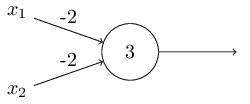
\includegraphics[width=0.4\textwidth]{simple_neuron}
\caption{A single neuron NAND gate with two identical weights, $w_1 = w_2 = -2$ and a bias $b = 3$}
\label{fig:simple_neuron}
\end{figure}

\noindent where \textit{b} is the so called bias of the neuron. With this definition, one can pick weights such that the neuron can model a NAND gate. Recall that a NAND gate is an inverted AND gate. Therefore we wish to take two inputs A and B and output NOT(A and B). Consider a neuron that takes two binary inputs $(x_1,x_2)$ and outputs a binary response according to the architecture in Figure \ref{fig:simple_neuron}. In this simple case, the weights and bias are trivial to choose. For example, if $(x_1,x_2)=(1,0)$ then we have

\begin{align*}
n\left(w_1x_1 + w_2x_2 + b\right) & = n\Big((-2)(1) + (-2)(0) + 3\Big) \\
& = n(1) \\
& = 1
\end{align*}

\noindent The other permutations of inputs clearly describe the properties of the function we wished to recreate. The natural question to ask is one of generality, how does a step function model complex time series data or classify animals in images? The answer lies in the organization of  many neurons and the resulting topology that is formed from the grouping.

\section{Architectures, Activation, and Assimilation}
\label{sec: three_As}

The \textit{architecture} of a neural network refers to the structure that exists between individual nodes of a network. This paper will be discussing \textit{feed-forward neural networks} (FFNNs). A FFNN consists of \textit{L} layers of neurons with each layer containing $n_l$ single neurons, where $l=1, 2, ..., L$. The first layer of neurons are called the input layer. This layer is unique in the sense that it does not compute, but only sends the initial information into the network. From this point, the information is sent from one layer to the next and each neuron in a succeeding layer will fire according to it's activation function and input signal from the preceding layer of neurons.

\begin{figure}[!htb]
\centering
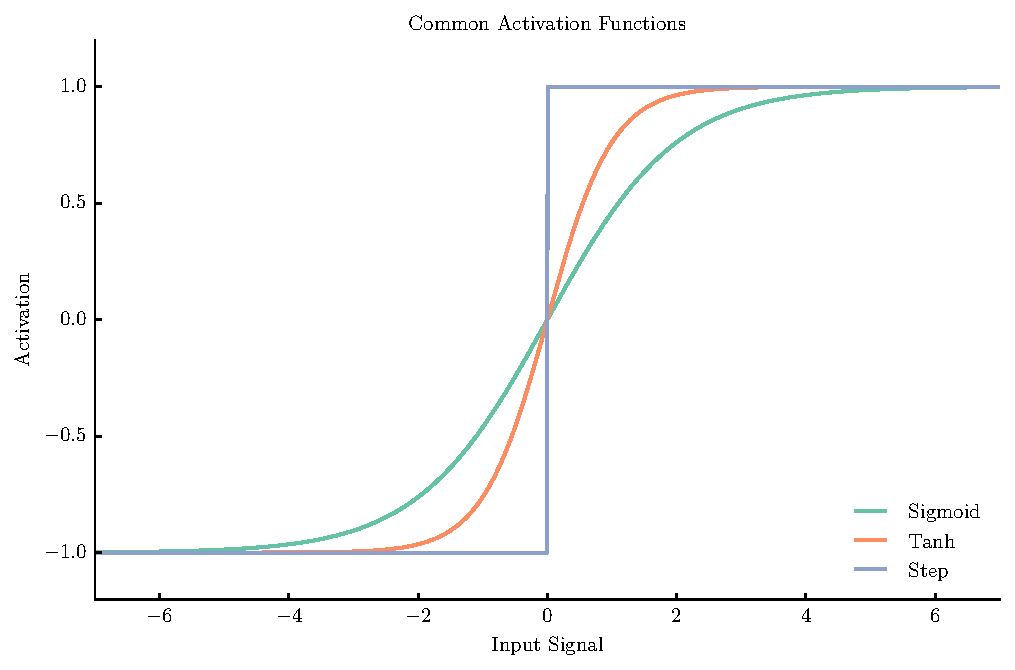
\includegraphics[width=\textwidth]{activation_functions.pdf}
\caption{Three common activation functions used in neural networks.}
\label{fig:act_fun}
\end{figure}

The \textit{activation function} of a FFNN refers to a non-linearity $\phi(\cdot)$ that is applied after the node receives a signal. For practical purposes, a smooth approximation to the step function is preferred. Hence $\phi$ is usually some sort of sigmodial function such as the logistic function or the tanh function (Figure \ref{fig:act_fun}). These functions have convenient analytic properties that one can take advantage of to train the network. The last layer of the network is called the output layer. This layer takes the signal from the last layer of hidden neurons and sends the signal through a final transfer function, which translates the output of the network to a result that can be understood within the context of the problem. Such transfer functions include an identity mapping (for regression) or a soft-max mapping for multi-label classification. FFNN neurons are all maximally connected. This means that every neuron in layer \textit{l} is connected to the neurons in layers $l - 1$ and $l + 1$. The network from Figure \ref{fig:simple_neuron} can be considered a FFNN with 0 hidden layers, 2 input neurons and 1 output neuron. More generally, the strength of connectivity between neuron \textit{j} in layer $l-1$ and neuron \textit{k} in layer $l$ is denoted by the weight $w^{l}_{jk}$ and neuron \textit{j} in layer \textit{l} carries a bias of $b^{l}_j$. One of the most interesting aspects of FFNNs is the ability to compute \textit{\textbf{any}} function with a single hidden layer of neurons. That is, given any function $f$ there exists a FFNN that can closely approximate \textit{f}. This is stated formally as the \textbf{Universal Approximation Theorem} (UAT).
%%%%%%%%%%%%%%%%%%%%%%%%%%%%%%%%%%%%%%%%%%%%%%%%%%%%%%%%%%%%%%%%%%%%%%%%%%%%%%%
\subsection{The Universal Approximation Theorem}
%%%%%%%%%%%%%%%%%%%%%%%%%%%%%%%%%%%%%%%%%%%%%%%%%%%%%%%%%%%%%%%%%%%%%%%%%%%%%%%
Let $g(\cdot)$ be a non-constant, bounded, and monotonically-increasing continuous function. Let $I_m$ denote the \textit{m}-dimensional unit hypercube $[0, 1]^m$. The space of continuous functions on $I_m$ is denoted by $C(I_m)$. Then, given any function $f\,\epsilon\,C(I_m)$ and $\epsilon > 0$, there exists an integer $n$, real constants $\alpha_i$, $\beta_i\,\epsilon\,\mathbb{R}$ and real vectors $\boldsymbol{\omega}_i \,\epsilon\,\mathbb{R}^m$, where $i=1,...,n$, such that we may define
%%%%%%%%%%%%%%%%%%%%%%%%%%%%%%%%%%%%%%%%%%%%%%%%%%%%%%%%%%%%%%%%%%%%%%%%%%%%%%%
\begin{equation*}
F(\textbf{x}) = \sum_{i=1}^{n} \alpha_i\,g(\boldsymbol{\omega}^T_i\textbf{x} + \beta_i)
\end{equation*}
%%%%%%%%%%%%%%%%%%%%%%%%%%%%%%%%%%%%%%%%%%%%%%%%%%%%%%%%%%%%%%%%%%%%%%%%%%%%%%%
as an approximate realization of the function \textit{f} where \textit{f} is independent of $g_i$; that is,
%%%%%%%%%%%%%%%%%%%%%%%%%%%%%%%%%%%%%%%%%%%%%%%%%%%%%%%%%%%%%%%%%%%%%%%%%%%%%%%
\begin{equation*}
|F(x) - f(x)| < \epsilon
\end{equation*}
%%%%%%%%%%%%%%%%%%%%%%%%%%%%%%%%%%%%%%%%%%%%%%%%%%%%%%%%%%%%%%%%%%%%%%%%%%%%%%%
for all $x\,\epsilon\,I_m$. In other words, functions of the form $F(x)$ are dense in $C(I_m)$. Furthermore, this theorem still holds when replacing $I_m$ with any compact subset of $\mathbb{R}^m$. 

While the \textit{rigorous} proof of the UAT is far beyond the scope of this manuscript, the following discussion will sketch how the UAT connects to FFNNs. Consider a FFNN with a single hidden layer with \textit{n} hidden neurons. For simplicity let the input be two dimensional and the output one dimensional. Let us denote these variables as $\textbf{x}=(x_1, x_2)$, and $y$. The first step to computing the signals $z_i$ into the hidden layer of neurons, where $i=1,2,...,n$
%%%%%%%%%%%%%%%%%%%%%%%%%%%%%%%%%%%%%%%%%%%%%%%%%%%%%%%%%%%%%%%%%%%%%%%%%%%%%%%
\begin{align*}
z_1 & = w^2_{11}x_1 + w^2_{21}x_2 + b^2_1 \\
z_2 & = w^2_{12}x_1 + w^2_{22}x_2 + b^2_2 \\
\vdots{}  \\
z_n & = w^2_{1n}x_1 + w^2_{2n}x_2 + b^2_n \\
\end{align*}
%%%%%%%%%%%%%%%%%%%%%%%%%%%%%%%%%%%%%%%%%%%%%%%%%%%%%%%%%%%%%%%%%%%%%%%%%%%%%%%
The hidden layer has a continuous output $a_i=\phi(z_i)$, where $\phi$ is a sigmoidal non-linearity. These activations are sent from the hidden layer to the output layer via the 2nd set of weights. Here, the final non-linearity is applied to give the output \textit{y}
%%%%%%%%%%%%%%%%%%%%%%%%%%%%%%%%%%%%%%%%%%%%%%%%%%%%%%%%%%%%%%%%%%%%%%%%%%%%%%%
\begin{equation*}
y = \psi\left(w^3_{11}a_1 + w^3_{21}a_2 + ... + w^3_{n1}a_n\right)
\end{equation*}
%%%%%%%%%%%%%%%%%%%%%%%%%%%%%%%%%%%%%%%%%%%%%%%%%%%%%%%%%%%%%%%%%%%%%%%%%%%%%%%
If $\psi$ is the identity mapping\footnote{This holds for all $\psi$, not just linear functions}, then we have exactly the construction of a function as shown in the UAT
%%%%%%%%%%%%%%%%%%%%%%%%%%%%%%%%%%%%%%%%%%%%%%%%%%%%%%%%%%%%%%%%%%%%%%%%%%%%%%%
\begin{align}
y & = w^3_{11}\phi({\textbf{w}^2_1}^T\textbf{x} + b^2_1) + ... + w^3_{n1}\phi({\textbf{w}^2_n}^T \textbf{x}+ b^2_n) \nonumber \\
& = \sum_{i=1}^{n} w^3_{i1}\phi({\textbf{w}^2_i}^T \textbf{x}+ b^2_i)
\end{align}
%%%%%%%%%%%%%%%%%%%%%%%%%%%%%%%%%%%%%%%%%%%%%%%%%%%%%%%%%%%%%%%%%%%%%%%%%%%%%%%
Therefore by the UAT the construction above will approximate any one dimensional function $f \, \in \, \mathbb{R}$.
%%%%%%%%%%%%%%%%%%%%%%%%%%%%%%%%%%%%%%%%%%%%%%%%%%%%%%%%%%%%%%%%%%%%%%%%%%%%%%%

The astute reader might be left with more questions at the end of the preceding analysis. How many hidden neurons does it take to approximate a function? How does one choose the weights and biases such that the approximation is a \textit{good} one? While the UAT guarantees the existence of such a network, little is claimed about how to go about constructing the architecture. The problem of choosing parameters becomes intractable as the number of hidden neurons increases. 

In a FFNN of one dimensional inputs and outputs, the number of adjustable parameters is given by $N_p=3n$, where \textit{n} is the number of hidden neurons in a single hidden layer. \textit{Deep neural networks} are often used to classify images. In the problem of digit classification, a network ingests an input image of size 28x28 which means the input space is 784 dimensional. The output space is 10 dimensional which corresponds to the 10 possible digits that can be recognized. Suppose further that a four layer FFNN is used to solve this problem. Even if there are only 10 neurons in each hidden layer, that corresponds to over 8000 adjustable weights and biases. Thus, in order to proceed we must consider an algorithmic way of optimizing these values to produce the \textit{best} network possible. This is referred to as the \textit{learning problem} in machine learning and it brings us to the final aspect of ANNs, assimilation.

\section{The Learning Problem} \label{learning_problem}

Suppose we are given a set of training examples $S=\lbrace(\textbf{x}_i, \textbf{y}_i), i=1,2,...,N| (\textbf{x}_i, \textbf{y}_i)\, \epsilon \, \mathbb{R}^{d_x} \times \mathbb{R}^{d_y}\rbrace$. The goal is to construct an \textit{L} layer FFNN that takes $\textbf{x}_i$ as an input and outputs an estimate $\boldsymbol{\eta}_i(\Theta)=\boldsymbol{\eta}(\textbf{x}_i| \Theta)$, where $\Theta=\lbrace \textbf{W}, \textbf{b} \rbrace$ is the set of weights and biases describing the network. We seek a parameter set $\Theta=\Theta^*$ such that $\boldsymbol{\eta}_i(\Theta^*)\approx\textbf{y}_i$. Since $\Theta$ is a random variable, $\Theta^*$ must be correspond to the parameter set that is most likely to be observed given what is known about the training data. We construct this probability distribution under the following assumptions. Assume each $\boldsymbol{\eta}_i$ is independent and identically distributed (i.i.d) and normally distributed around the target $\textbf{y}_i$. Furthermore, we constrain the weights to be normally distributed around \textbf{0} to avoid over-fitting of the training data and all biases are assumed to be drawn from a uniform distribution over some subset of the real line. Bayes Theorem can now be invoked to calculate the posterior distribution of $\Theta$ given the training examples
%%%%%%%%%%%%%%%%%%%%%%%%%%%%%%%%%%%%%%%%%%%%%%%%%%%%%%%%%%%%%%%%%%%%%%%%%%%%%%%
\begin{equation}
P(\Theta|S) = \frac{P(S|\Theta)P(\Theta)}{\int P(S|\Theta)P(\Theta) d\Theta}
\end{equation}
%%%%%%%%%%%%%%%%%%%%%%%%%%%%%%%%%%%%%%%%%%%%%%%%%%%%%%%%%%%%%%%%%%%%%%%%%%%%%%%
Maximizing this function is equivalent to minimizing $-ln\left[P(\Theta|S)\right]$. If we discard additive constants, the problem of maximizing $P(\Theta|S)$ transforms into the problem of minimizing the so called \textit{cost function}
%%%%%%%%%%%%%%%%%%%%%%%%%%%%%%%%%%%%%%%%%%%%%%%%%%%%%%%%%%%%%%%%%%%%%%%%%%%%%%%
\begin{equation}
E(\Theta|\textbf{X}) = \frac{1}{2N} \left[\boldsymbol{\eta}(\textbf{X}|\Theta) - \textbf{Y}\right] {\left[\boldsymbol{\eta}(\textbf{X}|\Theta) - \textbf{Y}\right]}^T \nonumber + \frac{\lambda}{2N_w}\sum_{l} \textbf{W}_l \textbf{W}_l^T
\label{cost_cost}
\end{equation}
%%%%%%%%%%%%%%%%%%%%%%%%%%%%%%%%%%%%%%%%%%%%%%%%%%%%%%%%%%%%%%%%%%%%%%%%%%%%%%%
The notation has been vectorized for brevity. \textbf{X} is the $N \times d_x$ input data matrix and \textbf{Y} is the $N \times d_y$ target data matrix. $\boldsymbol{\eta}(\textbf{X})$ is the output of the network, $N_w$ is the total number of weights, $\lambda$ is the regularization hyper-parameter, and $\textbf{W}_l$ are the matrix of weights connecting layers $l-1$ and $l$ such that each element of $\textbf{W}_l$ is $w^l_{jk}$. Now that we have a well defined objective in the learning problem, we discuss the algorithms used to find $\Theta^*$.
%%%%%%%%%%%%%%%%%%%%%%%%%%%%%%%%%%%%%%%%%%%%%%%%%%%%%%%%%%%%%%%%%%%%%%%%%%%%%%%
\subsection{Minimizing $E(\Theta)$}

In order to computationally minimize $E(\Theta)$ it is necessary to know the gradient of the cost with respect to all elements of $\Theta$. The \textit{back-propagation algorithm}, published in 1986 by \cite{rumelhart1988l} describes an algorithmic procedure for computing the gradient of the cost function. Note that for our network from section \ref{learning_problem} we have $\Theta=\lbrace \textbf{W}_2, \textbf{W}_3, ..., \textbf{W}_L, \textbf{b}_2, ..., \textbf{b}_{L} \rbrace$. Let us denote the inputs and outputs to layer $l$ as $\textbf{z}_l$ and $\textbf{a}_l$ respectively. The signals are related through the activation function\footnote{Note that the sum between the weighted components and the bias is broadcast row-wise.}
%%%%%%%%%%%%%%%%%%%%%%%%%%%%%%%%%%%%%%%%%%%%%%%%%%%%%%%%%%%%%%%%%%%%%%%%%%%%%%%
\begin{equation}
\textbf{a}_l = \psi(\textbf{z}_l), \, \textbf{z}_l = \textbf{a}_{l - 1}\textbf{W}_l + \textbf{b}_l
\end{equation}
%%%%%%%%%%%%%%%%%%%%%%%%%%%%%%%%%%%%%%%%%%%%%%%%%%%%%%%%%%%%%%%%%%%%%%%%%%%%%%%
Note that $\textbf{z}_1$ does not exist, as there is no signal going into layer 1, $\textbf{a}_L = \boldsymbol{\eta}(\textbf{X})$\footnote{The $\Theta$ has been suppressed here for brevity.}, and $\textbf{a}_1 = \textbf{X}$. The recursive structure of the network implies that derivatives in layer $l$ depend on layers \textit{ahead} of them. To see this note that for $l=L$ we have
%%%%%%%%%%%%%%%%%%%%%%%%%%%%%%%%%%%%%%%%%%%%%%%%%%%%%%%%%%%%%%%%%%%%%%%%%%%%%%%
\begin{equation*}
\frac{\partial E}{\partial \textbf{W}_L} = 
\frac{1}{N} \textbf{a}^T_{L - 1}
\left[\boldsymbol{\eta}(\textbf{X}) - \textbf{Y}\right] \odot
\psi^{\prime}(\textbf{z}_{L}) + \frac{\lambda}{N_w}\textbf{W}_L
\end{equation*}
%%%%%%%%%%%%%%%%%%%%%%%%%%%%%%%%%%%%%%%%%%%%%%%%%%%%%%%%%%%%%%%%%%%%%%%%%%%%%%%
\begin{equation*}
\frac{\partial E}{\partial \textbf{b}_L} = 
\frac{1}{N} \textbf{1}^T
\left[\boldsymbol{\eta}(\textbf{X}) - \textbf{Y}\right] \odot
\psi^{\prime}(\textbf{z}_{L})
\end{equation*}
%%%%%%%%%%%%%%%%%%%%%%%%%%%%%%%%%%%%%%%%%%%%%%%%%%%%%%%%%%%%%%%%%%%%%%%%%%%%%%%
Where $\odot$ represents the element-wise product, $\psi^{\prime}(\cdot)$ is the derivative of the transfer function applied element-wise, and \textbf{1} is a vector of 1's. Defining $\boldsymbol{\delta}_{L} = \frac{1}{N} \left[\boldsymbol{\eta}(\textbf{X}) - \textbf{Y}\right] \odot \psi^{\prime}(\textbf{z}_{L})$ we have
%%%%%%%%%%%%%%%%%%%%%%%%%%%%%%%%%%%%%%%%%%%%%%%%%%%%%%%%%%%%%%%%%%%%%%%%%%%%%%%
\begin{equation*}
\frac{\partial E}{\partial \textbf{W}_L} = 
\textbf{a}^T_{L - 1}\boldsymbol{\delta}_{L} + \frac{\lambda}{N_w}\textbf{W}_L
\end{equation*}
%%%%%%%%%%%%%%%%%%%%%%%%%%%%%%%%%%%%%%%%%%%%%%%%%%%%%%%%%%%%%%%%%%%%%%%%%%%%%%%
\begin{equation*}
\frac{\partial E}{\partial \textbf{b}_L} = 
\textbf{1}^T\boldsymbol{\delta}_{L}
\end{equation*}
%%%%%%%%%%%%%%%%%%%%%%%%%%%%%%%%%%%%%%%%%%%%%%%%%%%%%%%%%%%%%%%%%%%%%%%%%%%%%%%
A pattern reveals itself as we consider $l=L-1$
%%%%%%%%%%%%%%%%%%%%%%%%%%%%%%%%%%%%%%%%%%%%%%%%%%%%%%%%%%%%%%%%%%%%%%%%%%%%%%%
\begin{eqnarray*}
\frac{\partial E}{\partial \textbf{W}_{L - 1}} & = & 
\frac{1}{N} \textbf{a}^T_{L - 2}
\boldsymbol{\delta}_L \textbf{W}^T_L \odot
\psi^{\prime}(\textbf{z}_{L - 1}) + \frac{\lambda}{N_w}\textbf{W}_{L - 1} \nonumber \\
& = & \textbf{a}^T_{L - 2}
\boldsymbol{\delta}_{L - 1} + \frac{\lambda}{N_w}\textbf{W}_{L - 1}
\end{eqnarray*}
%%%%%%%%%%%%%%%%%%%%%%%%%%%%%%%%%%%%%%%%%%%%%%%%%%%%%%%%%%%%%%%%%%%%%%%%%%%%%%%
\begin{eqnarray*}
\frac{\partial E}{\partial \textbf{b}_{L - 1}} & = & 
\frac{1}{N} \textbf{1}^T
\boldsymbol{\delta}_L \textbf{W}^T_L \odot
\psi^{\prime}(\textbf{z}_{L - 1}) \nonumber \\
& = & \textbf{1}^T
\boldsymbol{\delta}_{L - 1}
\end{eqnarray*}
%%%%%%%%%%%%%%%%%%%%%%%%%%%%%%%%%%%%%%%%%%%%%%%%%%%%%%%%%%%%%%%%%%%%%%%%%%%%%%%
where $\boldsymbol{\delta}_{L - 1} = \frac{1}{N} \boldsymbol{\delta}_L \textbf{W}^T_L \odot \psi^{\prime}(\textbf{z}_{L - 1})$. This is extended by induction until $l = 2$ and we have the complete gradient of the cost function
%%%%%%%%%%%%%%%%%%%%%%%%%%%%%%%%%%%%%%%%%%%%%%%%%%%%%%%%%%%%%%%%%%%%%%%%%%%%%%%
\begin{equation}
\boldsymbol{\delta}_{l} = \frac{1}{N} \boldsymbol{\delta}_{l + 1} \textbf{W}^T_{l + 1} \odot \psi^{\prime}(\textbf{z}_{l})
\end{equation}
%%%%%%%%%%%%%%%%%%%%%%%%%%%%%%%%%%%%%%%%%%%%%%%%%%%%%%%%%%%%%%%%%%%%%%%%%%%%%%%
\begin{equation}
\frac{\partial E}{\partial \textbf{W}_{l}} = 
\textbf{a}^T_{l - 1}
\boldsymbol{\delta}_{l} + \frac{\lambda}{N_w}\textbf{W}_{l}
\end{equation}
%%%%%%%%%%%%%%%%%%%%%%%%%%%%%%%%%%%%%%%%%%%%%%%%%%%%%%%%%%%%%%%%%%%%%%%%%%%%%%%
\begin{equation}
\frac{\partial E}{\partial \textbf{b}_{l}} = \textbf{1}^T
\boldsymbol{\delta}_{l}
\end{equation}
%%%%%%%%%%%%%%%%%%%%%%%%%%%%%%%%%%%%%%%%%%%%%%%%%%%%%%%%%%%%%%%%%%%%%%%%%%%%%%%
Notice that $\boldsymbol{\delta}_l$ can be cast as a derivative of the cost with respect to the signal input to layer $l$, $\partial E/ \partial \textbf{z}_{l}$. Therefore, one can consider $\boldsymbol{\delta}_{l}$ as being a measure of the error in layer $l$ of the network. With this result, the back-propagation algorithm can be stated in its entirety.
%%%%%%%%%%%%%%%%%%%%%%%%%%%%%%%%%%%%%%%%%%%%%%%%%%%%%%%%%%%%%%%%%%%%%%%%%%%%%%%
\subsection{The Back-propagation Algorithm}
\label{backprop}
%%%%%%%%%%%%%%%%%%%%%%%%%%%%%%%%%%%%%%%%%%%%%%%%%%%%%%%%%%%%%%%%%%%%%%%%%%%%%%%
\begin{enumerate}[topsep=0pt,itemsep=0ex,partopsep=1ex,parsep=1ex]
\item Set $\textbf{a}_1 = \textbf{X}$
\item Compute $\textbf{z}_l = \textbf{a}_{l - 1}\textbf{W}_l + \textbf{b}_l$ and $\textbf{a}_l = \psi(\textbf{z}_l)$ for $l=2,3,...,L$
\item Compute $\boldsymbol{\delta}_L = \frac{1}{N} \left[\boldsymbol{\eta}(\textbf{X}) - \textbf{Y}\right] \odot \psi^{\prime}(\textbf{z}_{L})$
\item Compute $\boldsymbol{\delta}_{l} = \frac{1}{N} \boldsymbol{\delta}_{l + 1} \textbf{W}^T_{l + 1} \odot \psi^{\prime}(\textbf{z}_{l})$ for $l=L - 1, L - 2, ...., 2$
\item $\nabla E(\textbf{W}, \textbf{b})$ is given by $\frac{\partial E}{\partial \textbf{W}_{l}} = \textbf{a}^T_{l - 1} \boldsymbol{\delta}_{l} + \frac{\lambda}{N_w}\textbf{W}_{l}$, and $\frac{\partial E}{\partial \textbf{b}_{l}} = \textbf{1}^T \boldsymbol{\delta}_{l}$ for $l = L, L - 1, ..., 2$
\end{enumerate}

\noindent We can now use one of many gradient based optimization techniques to find the optimal parameters for the network. In all of the applications that follow, the Broyden - Fletcher - Goldfarb - Shanno (BFGS) algorithm is used to minimize the cost function. The BFGS method is a hill climbing technique that requires the Jacobian of the cost function (provided by the back-propagation algorithm). Given 0th and 1st order information, the algorithm implemented by the python library \texttt{scipy.optimize} also approximates the Hessian of the cost function. In practice BFGS converges significantly faster than batch gradient descent and hence is a favorable algorithm to use for the problems outlined in this study. Future work will include developing more complex algorithms to handle the minutiae of climate data.
%%%%%%%%%%%%%%%%%%%%%%%%%%%%%%%%%%%%%%%%%%%%%%%%%%%%%%%%%%%%%%%%%%%%%%%%%%%%%%%
%%%%%%%%%%%%%%%%%%%%%%%%%%%%%%%%%%%%%%%%%%%%%%%%%%%%%%%%%%%%%%%%%%%%%%%%%%%%%%%
\section{ANNs in Practice}
\label{ann_practice}
%
\subsection{Example: Nonlinear Fitting}

Consider the toy problem of fitting a one dimensional function. There are a multitude of existing techniques to solve this problem, the most common being linear regression. However, these models usually need a specific characterization of the function. Neural networks have the advantage of a fluid functional form. The architecture is the only information that needs to be fed into the system. There is an art in picking an optimal architecture, but many architectures are redundant and will model a training set equally well. In this example we sample 100 training and 100 testing points from the function
\begin{equation} \label{g}
g(x) = \exp(-x^2)\sin(5\pi x)
\end{equation}
for $x\in[-1, 1]$. This function has both changing amplitude and oscillatory structure, two important features that appear in many physical datasets. White noise is added to both sets of data to test the robustness of the network. The FFNN is set up with two hidden layers of 10, and 5 neurons respectively. See Figure \ref{fig:costReg} for a plot of the training process. Note that the generalization of the model is good, as there is little over-fitting of the training set. The resulting fit is shown in Figure \ref{fig:nnReg}. The model is an excellent fit for the testing data.
%
\subsection{Example: The Lorentz Model}
Next, we consider the dynamical problem of modeling differential equations. A \textit{Lorentz system} is a set of nonlinear coupled differential equations
\begin{equation}
\begin{pmatrix} 
\dot{x} \\
\dot{y} \\
\dot{z} \\
\end{pmatrix} 
=
\begin{pmatrix} 
\sigma (y - x) \\
x (\rho - z) - y \\
xy - \beta z \\
\end{pmatrix} 
\end{equation}
where $\dot{u} = du/ dt$. The Lorentz system is characterized by having chaotic solutions and large sensitivities to initial conditions. The \textit{Lorentz attractor} is a particular set of solutions, made famous by it's resemblance to a butterfly in 3-space (See Figure \ref{fig:3d Lorentz}). In this example, the vertical dynamical component is replaced by a FFNN
\begin{equation}
\begin{pmatrix} 
\dot{x} \\
\dot{y} \\
\dot{z} \\
\end{pmatrix} 
=
\begin{pmatrix} 
\sigma (y - x) \\
x (\rho - z) - y \\
\mathcal{N} \\
\end{pmatrix}
\end{equation}
where $\mathcal{N}=\mathcal{N}(x, y, z, \dot{x}, \dot{y})$. 

We first run the complete Lorentz system for a total time of 16 units. The system is integrated using a 4th order Runge-Kutta scheme with parameters $(\sigma, \rho, \beta)=(0, 8/3, 28)$ and an initialization of $(x_0, y_0, z_0)=(1.508870, -1.531271, 25.46091)$. These conditions result in a strange attractor solution. Figure \ref{fig:2d Lorentz} is a component plot of the solution. The multi-modal nature of the system is quite obvious, having an approximate period of five seconds. This feature is visualized in 3-space by the two winged structure of the attractor. After experimenting with different layer architectures, a single hidden layer with 50 neurons was found to have the best fit. Plots of the cost functions and the residual errors are shown in Figures \ref{fig:costs Lorentz} and \ref{fig:nn Lorentz}. The costs have been minimized and the generalization error is relatively low. However, the network is clearly having trouble following the trajectory of the model. This first starts occurring approximately five seconds into the simulation, corresponding with a change in mode. The network continues the simulation assuming the model should still be in the first mode. 

This is symptomatic of a larger problem concerning FFNNs. The network does not have any internal memory, meaning that it cannot assimilate temporal information. Which is paramount to understanding how the model oscillates between modes. If the number of neurons in the hidden layer are increased, the network tracks the model further. However, the network will always eventually lose the signal after a certain number of mode changes. In order to further improve statistical performance, a new type of architecture must be considered. \textit{Recurrent neural networks} (RNNs) are a class of ANNs that have been shown to better constrain highly non-linear time series \cite{seidl1991}. RNNs have connections between neurons that are closed cycles. The architecture gains a notion of memory, where information from previous time steps can be fed back into the network to further constrain the model.
\begin{figure}[!htb]
\centering
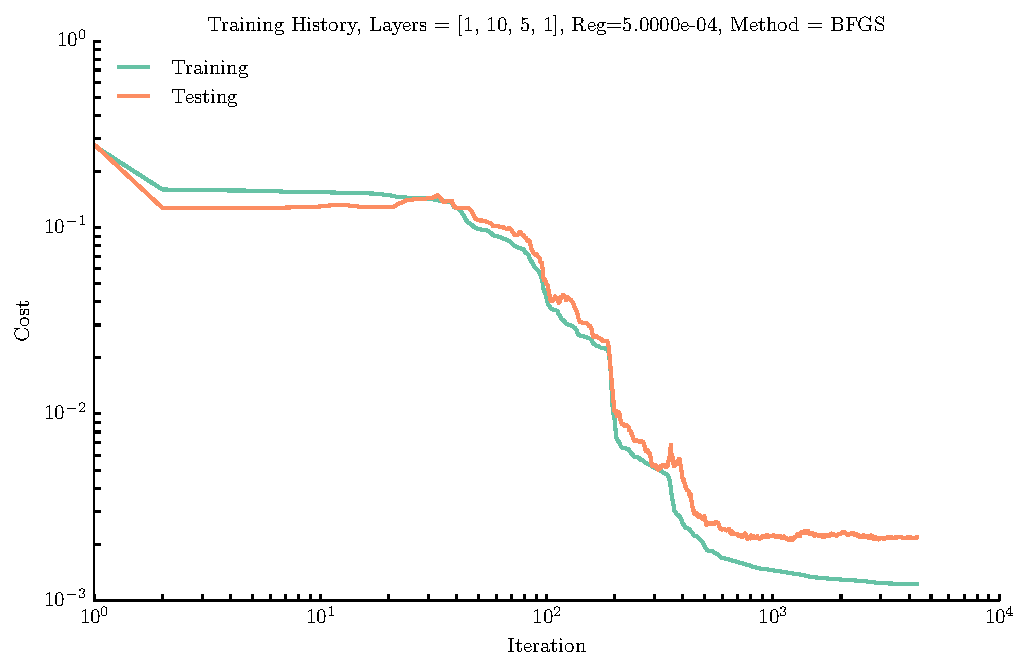
\includegraphics[width=\textwidth]{costs.pdf}
\caption{Plots of the cost function during the training of the FFNN. Note the minimal over-fitting illustrated by the testing cost curve.}
\label{fig:costReg}
\end{figure}
\begin{figure}[!htb]
\centering
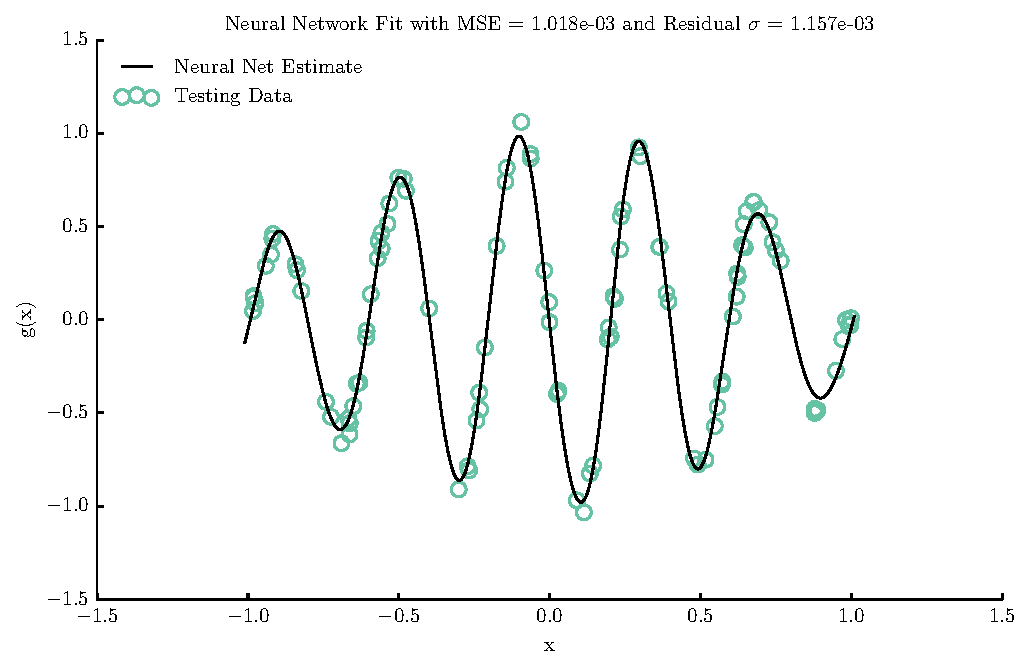
\includegraphics[width=\textwidth]{nnReg.pdf}
\caption{The neural network fit of equation \ref{g}.}
\label{fig:nnReg}
\end{figure}
\begin{figure}[!htb]
\centering
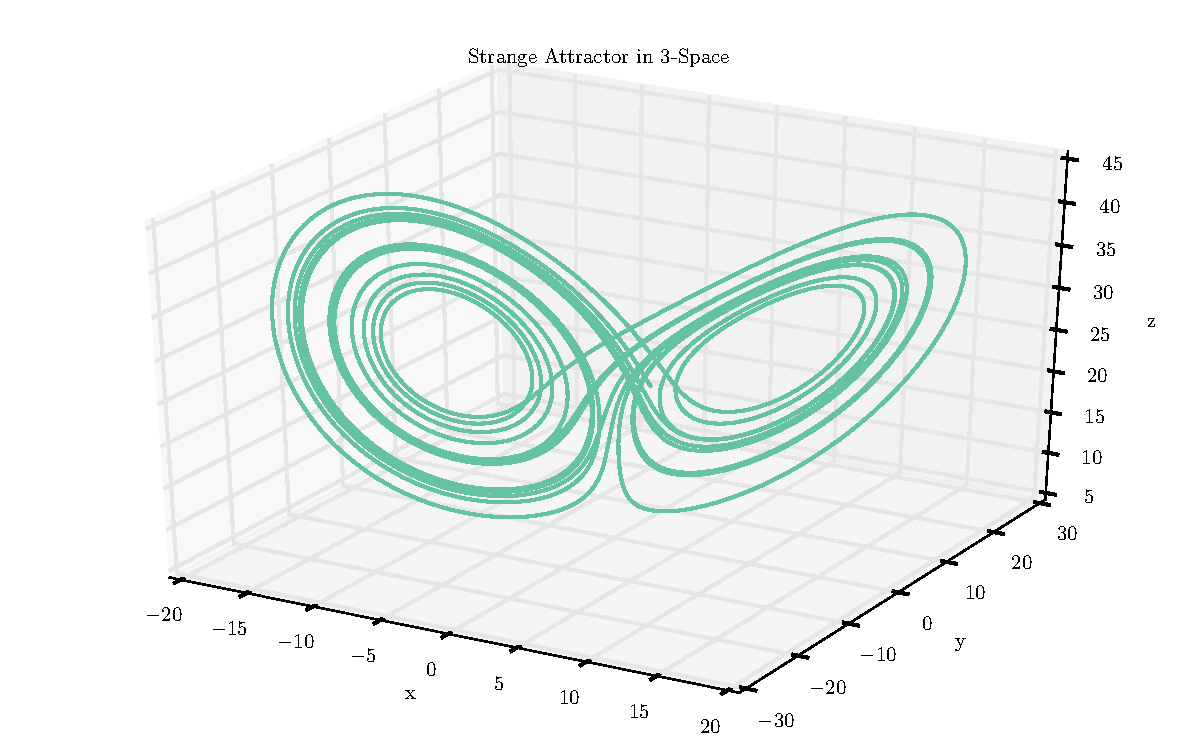
\includegraphics[width=\textwidth]{3dLorentz.pdf}
\caption{The strange attractor solution to the Lorentz system.}
\label{fig:3d Lorentz}
\end{figure}
\begin{figure}[!htb]
\centering
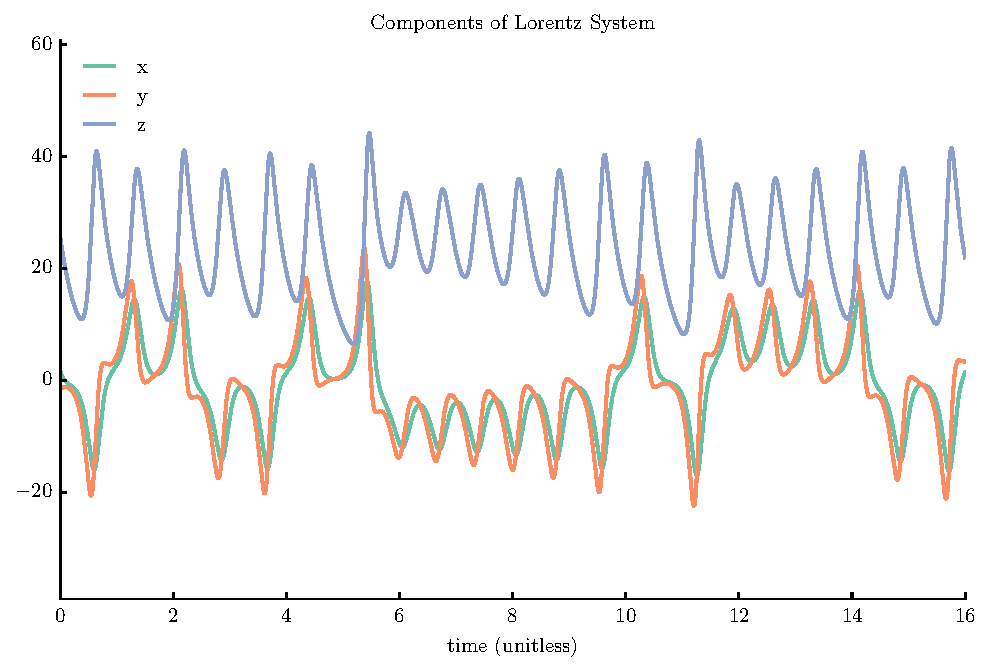
\includegraphics[width=\textwidth]{2dLorentz.pdf}
\caption{The individual components for the strange attractor solution. There is a unique multi-modal structure in which the solution persists between the two modes.}
\label{fig:2d Lorentz}
\end{figure}
\begin{figure}[!htb]
\centering
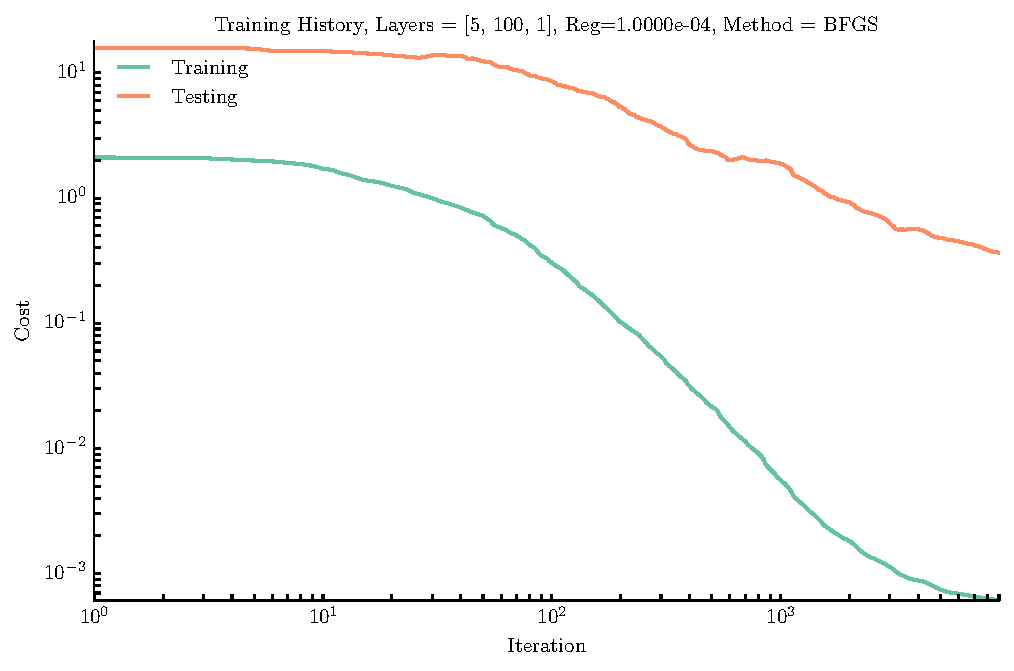
\includegraphics[width=\textwidth]{costsLorentz.pdf}
\caption{The cost function history for training the Lorentz network. The minimal over-error near the end is relatively negligible.}
\label{fig:costs Lorentz}
\end{figure}
\begin{figure}[!htb]
\centering
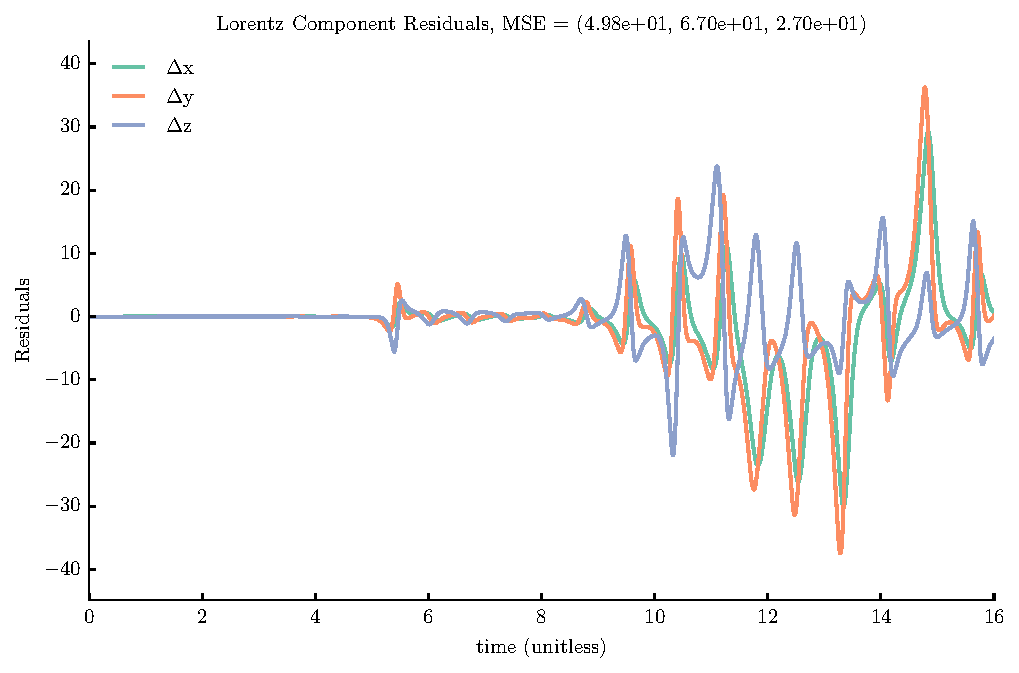
\includegraphics[width=\textwidth]{lorentz_solution.pdf}
\caption{The residuals between the trained network and the true dynamical state of the Lorentz system. The network has a good fit until the mode changes, where it loses track of the solution and errors start to accumulate quickly.}
\label{fig:nn Lorentz}
\end{figure}